% !TeX root = ../libro.tex
% !TeX encoding = utf8

\chapter{AutoLoops}

Como ejemplo de aplicación del contenido teórico del trabajo se ha desarrollado la herramienta AutoLoops, basada en el modelo MusicVAE de Magenta. Permite la manipulación sencilla del espacio latente de melodías de dos compases, permitiendo la codificación de una melodía ya existente y la exploración del espacio cercano para la generación de nuevos ejemplos relacionados.

La herramienta se inspira en las múltiples demostraciones ya  disponibles en la web que implementan los modelos desarrollados por Magenta, pero con pretensión de aplicación al proceso real de composición musical. Desde su concepción inicial se establece no solo como un ejemplo de las capacidades del modelo, sino también como una herramienta que pueda ser utilizada directamente por artistas en el contexto real de la composición y producción musical.

En cuanto a su utilización, la herramienta se basa en el método de trabajo que muchas veces se utiliza para el diseño sonoro en los sintetizadores. Estos permiten la generación y modificación de ondas sonoras para la creación de timbres. Muchas veces es difícil entender la repercusión exacta que tendrá en el sonido producido la modificación de alguna de estas características, o la interacción entre varias de estas modificaciones. Es por ello que muchas veces la construcción de un sonido se realiza explorando el espacio que las características ofrecen mediante el método de prueba y error.

Se trata por tanto de traducir este método al trabajo con melodías. Mediante el modelo MusicVAE (\autoref{modelo}) se obtienen las características de una melodía, aunque su significado es oculto. El artista puede cargar su propia melodía y generar nuevas a partir de la misma modificando las características que se le proporcionan. Podrá generar una secuencia de melodías de dos compases o una sola melodía que podrá exportar como archivo MIDI, que puede usarse en la producción de una canción.

\begin{figure}[htpb]
  \centering
  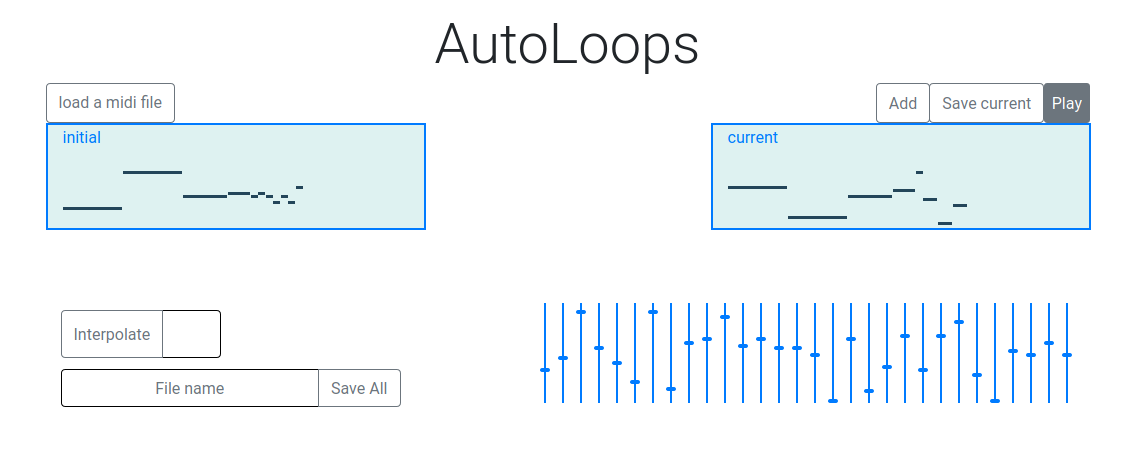
\includegraphics[width=1.1\textwidth]{autoloops}
  \caption{Interfaz de AutoLoops}
  \label{fig:autoloops}
\end{figure}

\section{Marco de trabajo}

La herramienta se ha desarollado en forma de aplicación web para la que se ha utilizado HTML y CSS para el diseño de la interfaz y JavaScript para el funcionamiento interno.

\subsection{HTML}

Para la maquetación de la interfaz se ha utilizado HTML, lenguaje de marcado estándar a cargo del \textit{World Wide Web Consortium} (W3C). Sobre este se ha utilizado la biblioteca Bootstrap para el diseño con sistema de rejilla. Puede incluirse dicha biblioteca mediante la siguiente línea en la cabecera.

\begin{lstlisting}
<link rel="stylesheet" href="https://stackpath.bootstrapcdn.com/bootstrap/4.5.2/css/bootstrap.min.css">
\end{lstlisting}

Además también se ha utilizado una hoja de estilos CSS.

\subsection{CSS}

Mientras que HTML tiene el contenido de la interfaz, la hoja CSS contiene el diseño de los elementos de la misma. Para su inclusión se debe añadir la siguiente línea en la cabecera.

\begin{lstlisting}
<link rel="stylesheet" href="assets/css/index.css">
\end{lstlisting}

\subsection{JavaScript}

Para la programación del funcionamiento de la aplicación se utiliza JavaScript, un lenguaje de programación interpretado utilizado principalmente en páginas web y aplicaciones de servidor. Para exportar los archivos MIDI necesarios se ha utilizado la biblioteca FileSaver, que se incluye mediante la siguiente línea en la cabecera del archivo HTML.

\begin{lstlisting}
<script src="https://cdnjs.cloudflare.com/ajax/libs/FileSaver.js/1.3.8/FileSaver.min.js" defer></script>
\end{lstlisting}

Para la visualización de datos se utiliza la biblioteca D3, que se incluye mediante la siguiente línea en la cabecera del archivo HTML.

\begin{lstlisting}
<script src="https://cdnjs.cloudflare.com/ajax/libs/d3/5.15.0/d3.js"></script>
\end{lstlisting}

Por último, y aquella con uso más extensivo por ser la que aporta el núcleo de la funcionalidad del programa, se ha utilizado la biblioteca Magenta.js.

\subsection{Biblioteca Magenta.js}

La biblioteca Magenta.js provee al desarrollador de una API de alto nivel para la aplicación de modelos de aprendizaje automático, especialmente aprendizaje profundo, para el modelado y manipulación de datos relacionados con el arte como imágenes y música. Está desarrollada sobre TensorFlow, una biblioteca para la creación de modelos de aprendizaje automático~\cite{magentajs}.

El paquete \textit{magenta/music} contiene una API para JavaScript para la interacción con modelos para la generación de música. Puede incluirse añadiendo la siguiente línea en la cabecera del archivo HTML.

\begin{lstlisting}
<script src="https://cdn.jsdelivr.net/npm/@magenta/music@1.12.1/dist/magentamusic.min.js"></script>
\end{lstlisting}

El paquete contiene dos funcionalidades principales: procesamiento de datos y API para modelos, incluídos modelos pre-entrenados.

\subsubsection{Procesamiento de datos}

Se establece la clase $\textit{NoteSequence}$ como representación de partituras musicales. Esta representación almacena aspectos fundamentales de una secuencia de notas como son tiempos, tonos e instrumentos, pero también metadatos como etiquetas de secciones o información sobre acordes. El paquete también contiene una re-implementación de la librería $\textit{NoteSequence}$ de Magenta Python, que incluye funcionalidades para convertir MIDI en $\textit{NoteSequence}$ y viceversa, así como para la síntesis y reproducción de sonido. También existe la posibilidad de convertir las $\textit{NoteSequence}$ en tensores de la biblioteca TensorFlow, que son utilizados como entrada y salida de los modelos.

\subsubsection{Interfaces de modelos}

La biblioteca también incluye interfaces para los múltiples modelos de Magenta. Entre los modelos dedicados a la música se encuentran interfaces para MusicRNN~\cite{performance-rnn-2017}, MidiMe~\cite{midime}, Piano Genie~\cite{pianogenie}, GANSynth~\cite{engel2019gansynth}, y el modelo que se utiliza en este proyecto, MusicVAE.

Con respecto a este último modelo se implementan métodos que incluyen \textit{encode} y \textit{decode} para codificar \textit{NoteSequence} en vectores latentes y al revés. Además se añaden los métodos \textit{interpolate} para facilitar la operación de interpolación entre melodías (\autoref{interpolate}) y \textit{sample} para generar muestras de melodías.

Para evitar que el desarrollador tenga que llevar a cabo la costosa operación del entrenamiento del modelo se facilitan también archivos con los pesos del modelo. Estos se facilitan en forma de archivos de configuración JSON. En este caso utilizamos el modelo de MusicVAE para melodías de dos compases, por lo que cargamos el modelo mediante

\begin{lstlisting}
const model = new mm.MusicVAE('https://storage.googleapis.com/magentadata/js/checkpoints/music_vae/mel_2bar_small');
\end{lstlisting}

\section{Uso de la aplicación}

Para abrir la aplicación el usuario solo debe descargar los archivos y abrir $\textit{index.html}$ con un navegador. Hecho esto se visualizará la interfaz de la  \autoref{fig:autoloops}.

Para comenzar a utilizar la herramienta el usuario deberá cargar una melodía en formato MIDI monofónica de dos compases. Esta acción puede llevarse a cabo mediante el botón \textit{load a midi file}, que permitirá elegir el archivo sobre el que se quiere trabajar. Una vez la melodía ha sido introducida se mostrará en los cuadros \textit{initial} y \textit{current}.

\begin{figure}[htpb]
  \centering
  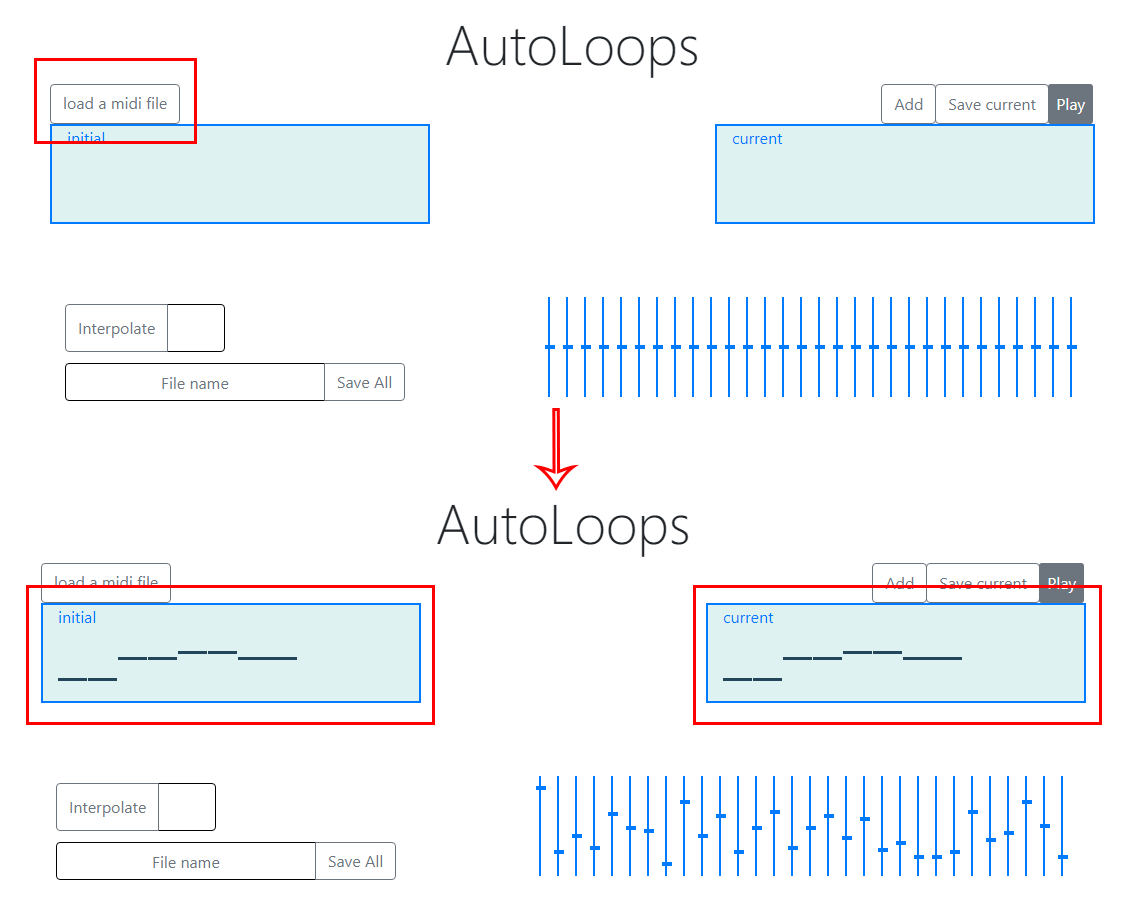
\includegraphics[width=1.1\textwidth]{loadmelody}
  \caption{Cargar una melodía a AutoLooops}
  \label{fig:loadmelody}
\end{figure}


Una vez la melodía está cargada puede comenzarse a generar nuevas melodías a partir de la misma. Los controles deslizantes reflejarán las características en el espacio latente de la melodía que se ha cargado. El usuario puede modificarlas y con ello se generarán nuevas melodías. El cambio podrá apreciarse visualmente en el cuadro \textit{current}, que mostrará la melodía correspondiente a la codificación actual marcada por los controles deslizantes. La melodía actual podrá también escucharse mediante el botón \textit{play}.

\begin{figure}[htpb]
  \centering
  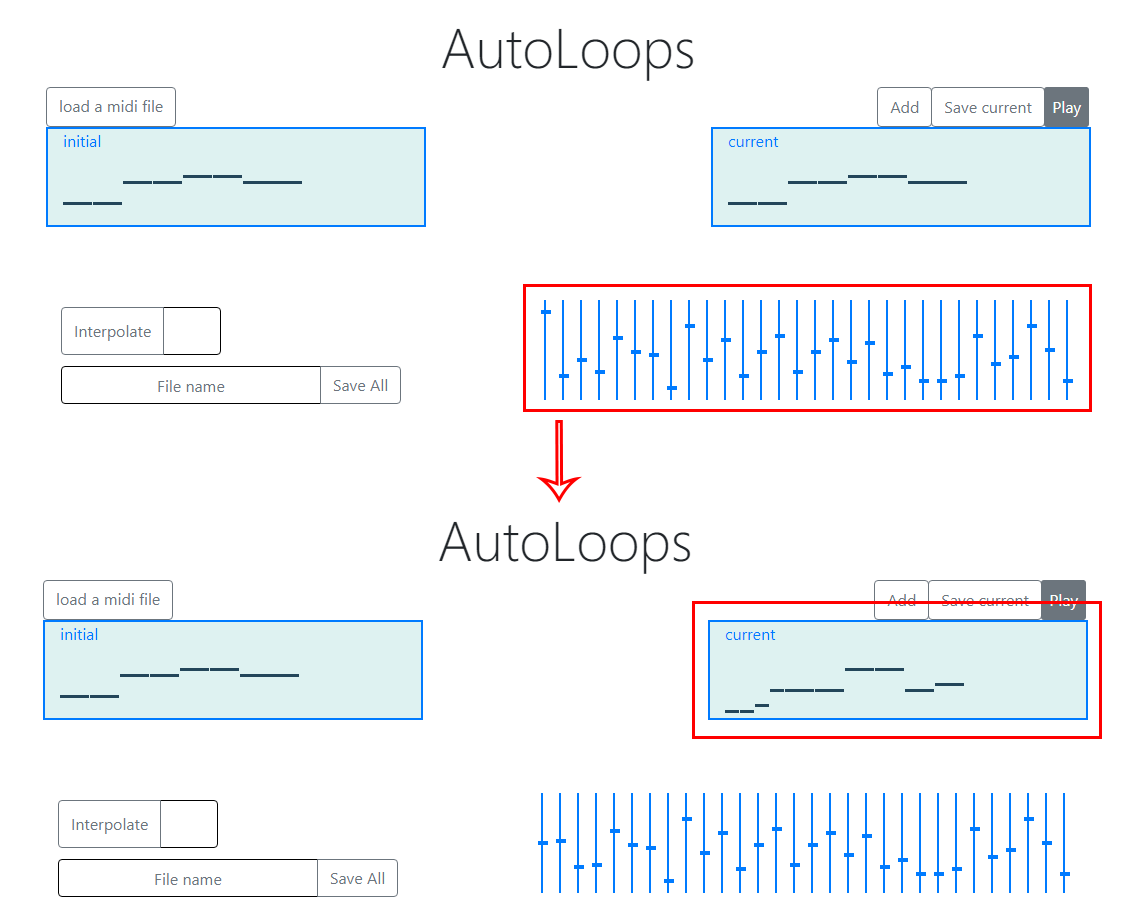
\includegraphics[width=1.1\textwidth]{changemelody}
  \caption{Crear una nueva melodía a AutoLooops}
  \label{fig:changemelody}
\end{figure}

Cada vez que el usuario lo considere oportuno puede utilizar el botón \textit{add} para guardar la melodía actual. Estas melodías guardadas podrán ser después exportadas como una secuencia completa mediante el botón \textit{save all}, que también cuenta con un campo para recoger el nombre para el archivo MIDI en el que se exportarán las melodías.

\begin{figure}[htpb]
  \centering
  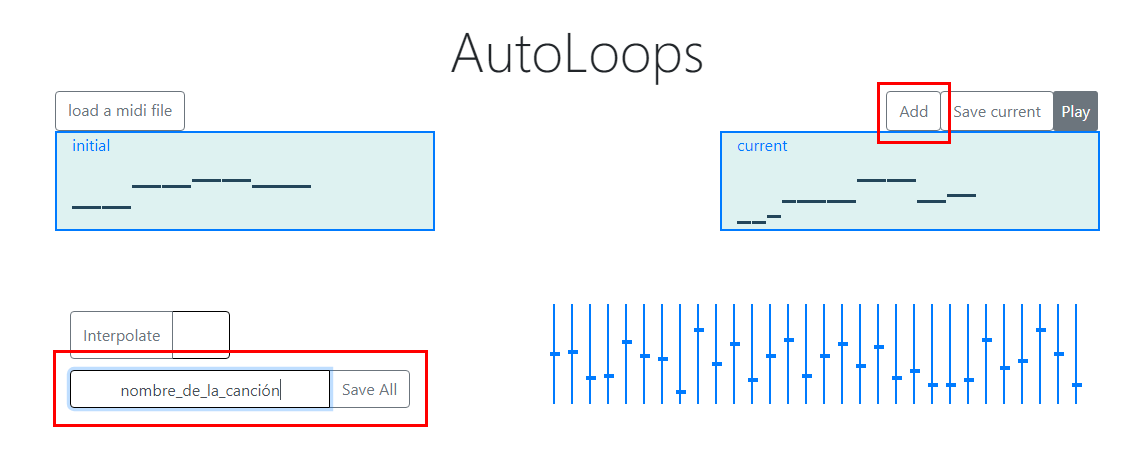
\includegraphics[width=1.1\textwidth]{savemelody}
  \caption{Guardar y exportar una secuencia de melodías en AutoLoops}
  \label{fig:savemelody}
\end{figure}

También puede exportarse únicamente la melodía actual mediante el botón \textit{save current}.

\begin{figure}[htpb]
  \centering
  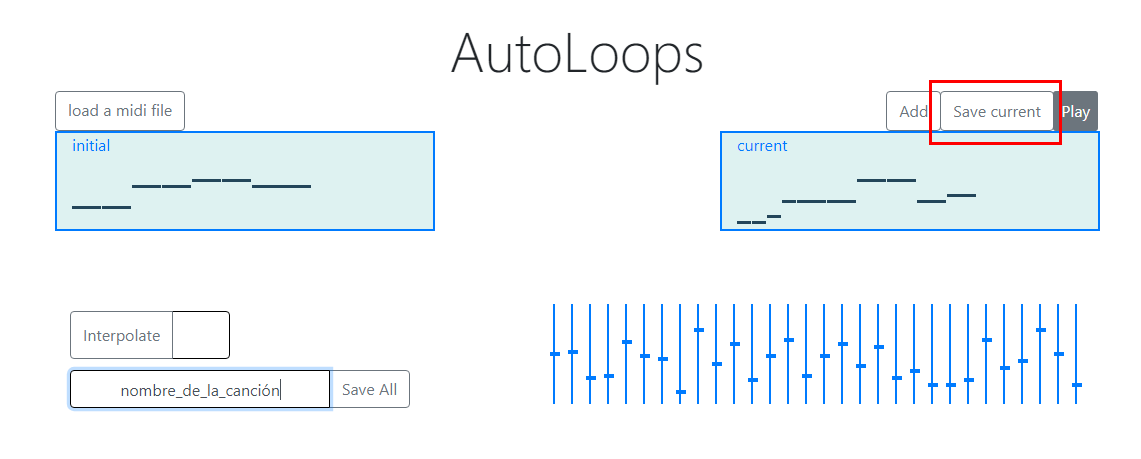
\includegraphics[width=1.1\textwidth]{savecurrentmelody}
  \caption{Exportar la melodía actual en AutoLoops}
  \label{fig:savecurrentmelody}
\end{figure}

Por último se ofrece también la posibilidad de interpolar entre la melodía actual y la melodía inicial. Para ello se hará uso del botón \textit{interpolate}, junto al que se incluye un campo para recoger el número de pasos que se quieren realizar. El usuario puede introducir un número y se guardará una interpolación entre la melodía de \textit{current} y la de \textit{initial} con ese número de melodías, siendo la primera de la secuencia la melodía actual y la última la melodía inicial. Hecho esto la melodía inicial pasará a ser la actual y puede proseguirse con la utilización del programa.

\begin{figure}[htpb]
  \centering
  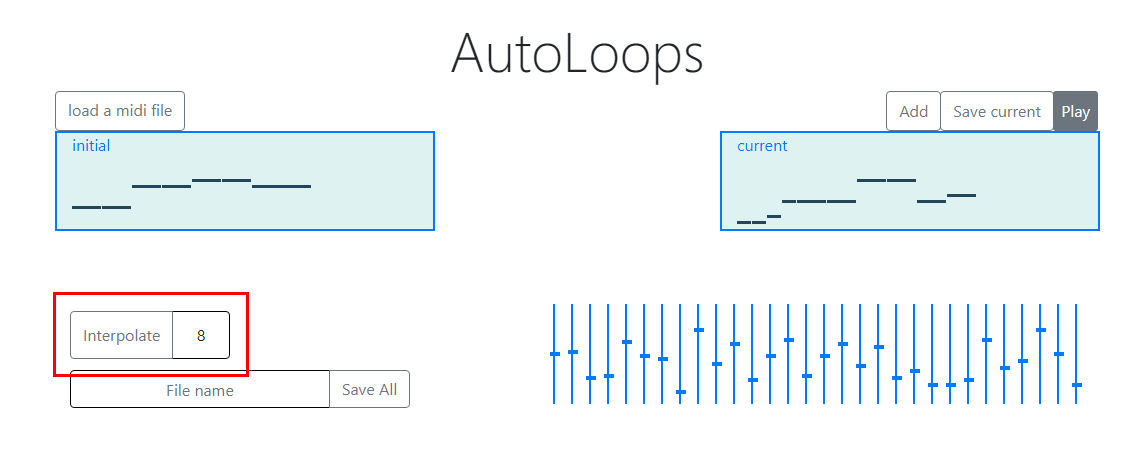
\includegraphics[width=1.1\textwidth]{interpolatemelody}
  \caption{Intepolación entre la melodía actual y la inicial en 8 pasos}
  \label{fig:savemelody}
\end{figure}

\section{Funcionamiento interno}

Comprendida la estructura general del programa puede detallarse su funcionamiento. Cuando el usuario carga una melodía MIDI se utiliza el método \textit{blobToNoteSequence} facilitado por la biblioteca \textit{magenta music} para convertir la secuencia cargada en un objeto del tipo \textit{NoteSequence}, que es la representación de melodías con las que se trata. Se utiliza entonces el modelo de MusicVAE para obtener la codificación de la melodía mediante el método \textit{encode}. Con la codificación obtenida se actualizan los controles deslizantes, haciendo que su posición corresponda al valor de la variable latente correspondiente. Hecho esto se decodifica la melodía mediante el método \textit{decode} y se toma dicha decodificación como melodía inicial y melodía actual. Por último se visualizan las melodías mediante el método \textit{PianoRollSVGVisualizer}, también de la biblioteca \textit{magenta music}.

Una vez establecidas las melodías inicial y actuales pueden moverse los controles deslizantes. Cualquier movimiento se captura y se maneja, creando un tensor con los valores modificados y decodificando dicho tensor para obtener la melodía actual.

Cada vez que se pulsa \textit{add} la melodía actual es añadida a las melodías ya guardadas. Se cuenta con una instancia de \textit{NoteSequence} para almacenar estas melodías. Cada vez que se concatena la que contiene las guardadas con la actual. Esta acción se realiza mediante el método \textit{concatenate} de \textit{magenta music}.

Cuando el usuario pulsa el botón \textit{save all} las melodías guardadas son exportadas a un archivo MIDI del nombre que el usuario elija. Para ello primero se transforma la melodía de \textit{NoteSequence} a MIDI mediante el método \textit{sequenceProtoToMidi} de \textit{magenta music}. Hecho esto el archivo se guarda mediante la función \textit{saveAs} de la biblioteca \textit{FileSaver}. De la misma manera cuando se pulsa \textit{save current} se transforma solo la melodía actual y se exporta.

Para realizar la interpolación se utiliza el método \textit{interpolate} correspondiente al modelo MusicVAE. Se toma como primera melodía de la interpolación la melodía actual y como última la melodía inicial, y se generan una secuencia de tantos pasos como los indicados por el usuario. Hecho esto cada elemento de la secuencia se añade a las secuencias guardadas.

\endinput
%------------------------------------------------------------------------------------
% FIN DEL CAPÍTULO.
%------------------------------------------------------------------------------------
